\documentclass[10pt]{beamer}

\usetheme[progressbar=frametitle]{metropolis}

\usepackage{amsmath}
\usepackage{amsthm}
\usepackage{amssymb}
\usepackage{appendixnumberbeamer}
\usepackage{booktabs}
\usepackage[scale=2]{ccicons}
\usepackage{pgfplots}
\usepgfplotslibrary{dateplot}
\usepackage{xspace}
\usepackage{graphicx}
\usepackage{subcaption}
\usepackage{bbm}

\newcommand{\themename}{\textbf{\textsc{metropolis}}\xspace}

\title{Authorship Verification}
\subtitle{Masters Thesis}
\date{}
\author{August S\o rensen \& Magnus Stavngaard}
\institute{University of Copenhagen}

\defbeamertemplate{description item}{align left}{\insertdescriptionitem\hfill}

\begin{document}

\maketitle

\begin{frame}[fragile]{Problem Statement}
    \begin{itemize}
        \item We catch ghostwriters.
    \end{itemize}
\end{frame}

\begin{frame}[fragile]{Solution Architecture}
    \begin{center}
        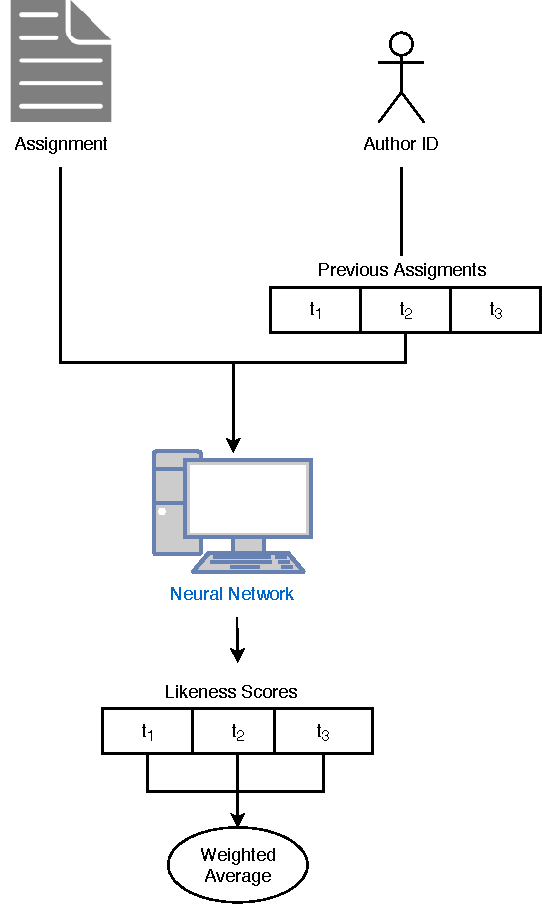
\includegraphics[width=0.45\textwidth]{../../macom/summary/pictures/Model}
    \end{center}
\end{frame}

\begin{frame}[fragile]{Siamese Networks}
    \begin{itemize}
        \item Siamese Neural Networks compares two objects.

            \begin{description}
                \item[Input] Two objects,
                \item[Output] Probability that objects belong to same class.
            \end{description}
    \end{itemize}

    \begin{center}
        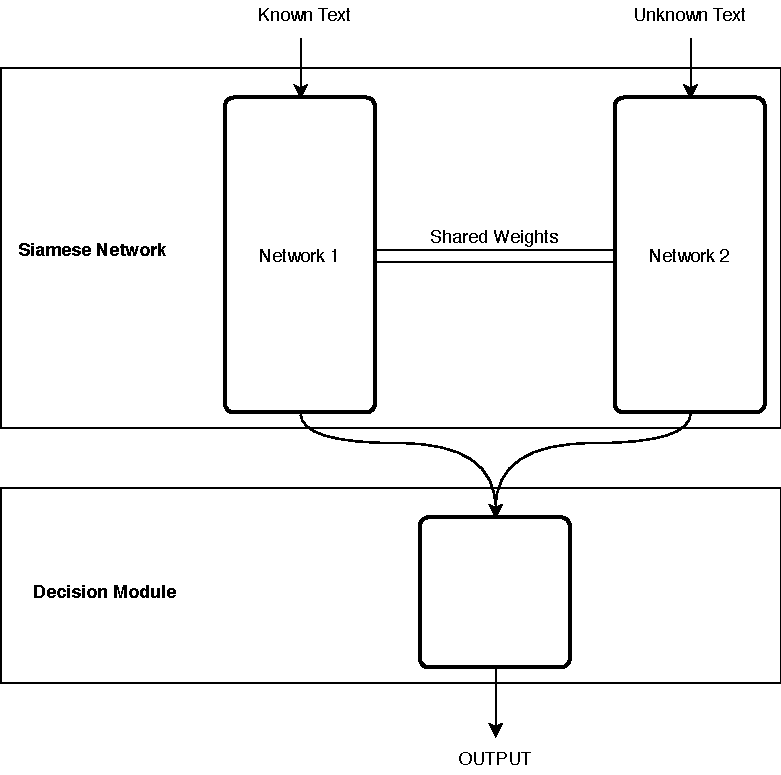
\includegraphics[width=0.6\textwidth]{../../report/pictures/method/siamese}
    \end{center}
\end{frame}

\begin{frame}[fragile]{Networks}
    \setbeamertemplate{description item}[align left]
    \begin{itemize}
        \item Networks consist of 4 parts:

            \begin{description}
                \item[Embedding] Encode raw texts in format suiting networks.
                \item[Feature Extraction] Extract feature vectors from the
                    encoded texts.
                \item[Combining] Combine extracted feature vectors using some
                    function.
                \item[Decision] Decide the probability that two texts are from
                    the same author.
            \end{description}
    \end{itemize}
\end{frame}

\begin{frame}[fragile]{Char-CNN}
    \begin{center}
        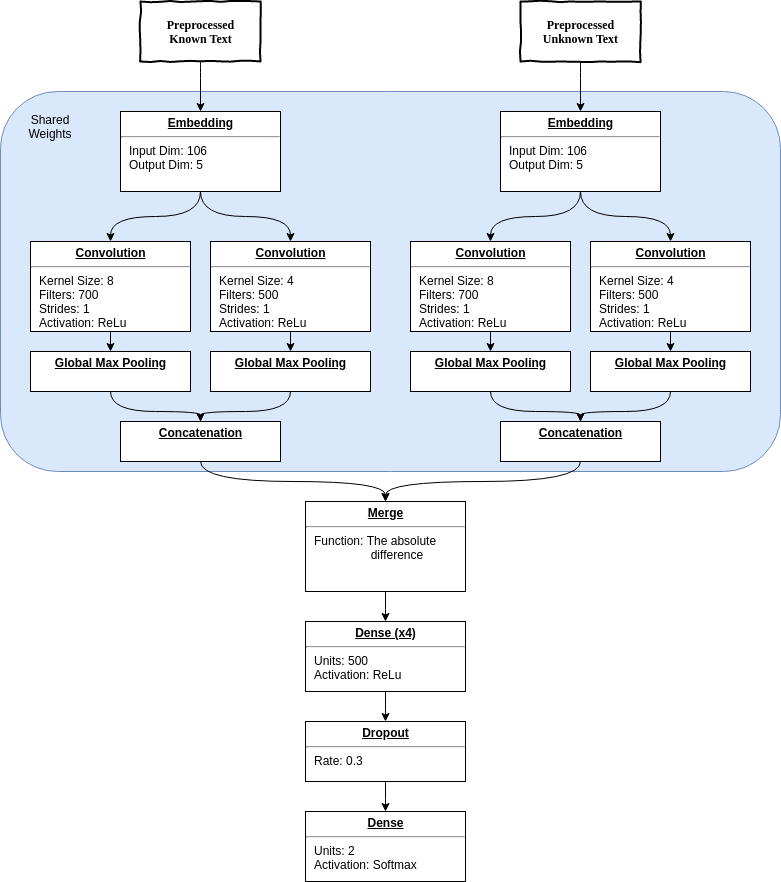
\includegraphics[width=0.6\textwidth]{../../report/pictures/experiments/conv_char_nn/model}
    \end{center}
\end{frame}

%\begin{frame}[fragile]{Sent-RNN}
    %\begin{center}
        %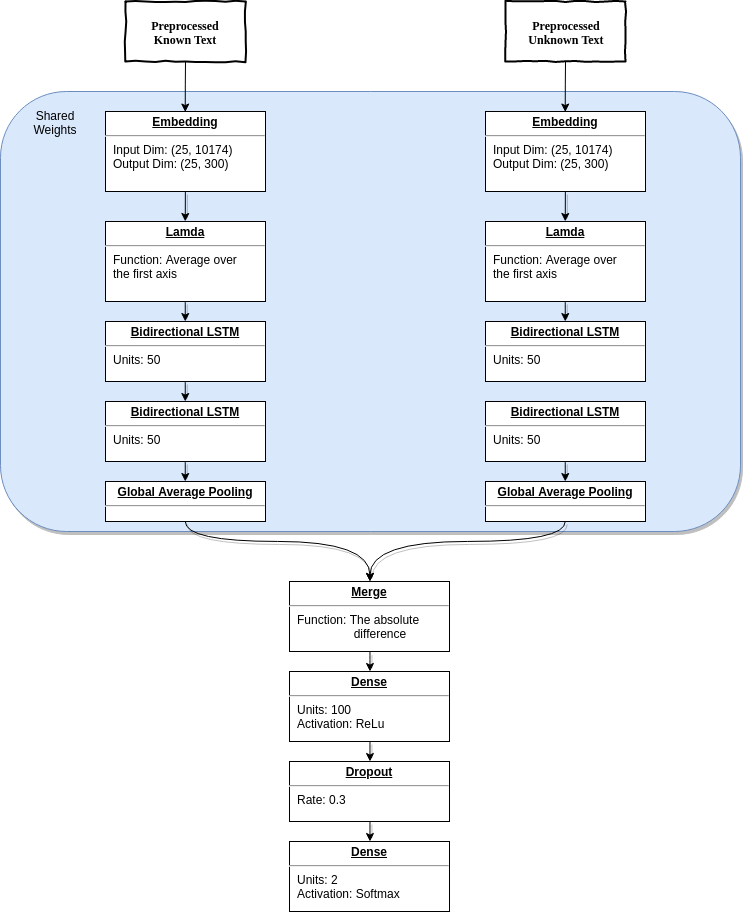
\includegraphics[width=0.6\textwidth]{../../report/pictures/experiments/rec_sent_nn/model}
    %\end{center}
%\end{frame}

%\begin{frame}[fragile]{Char-word-CNN}
    %\begin{center}
        %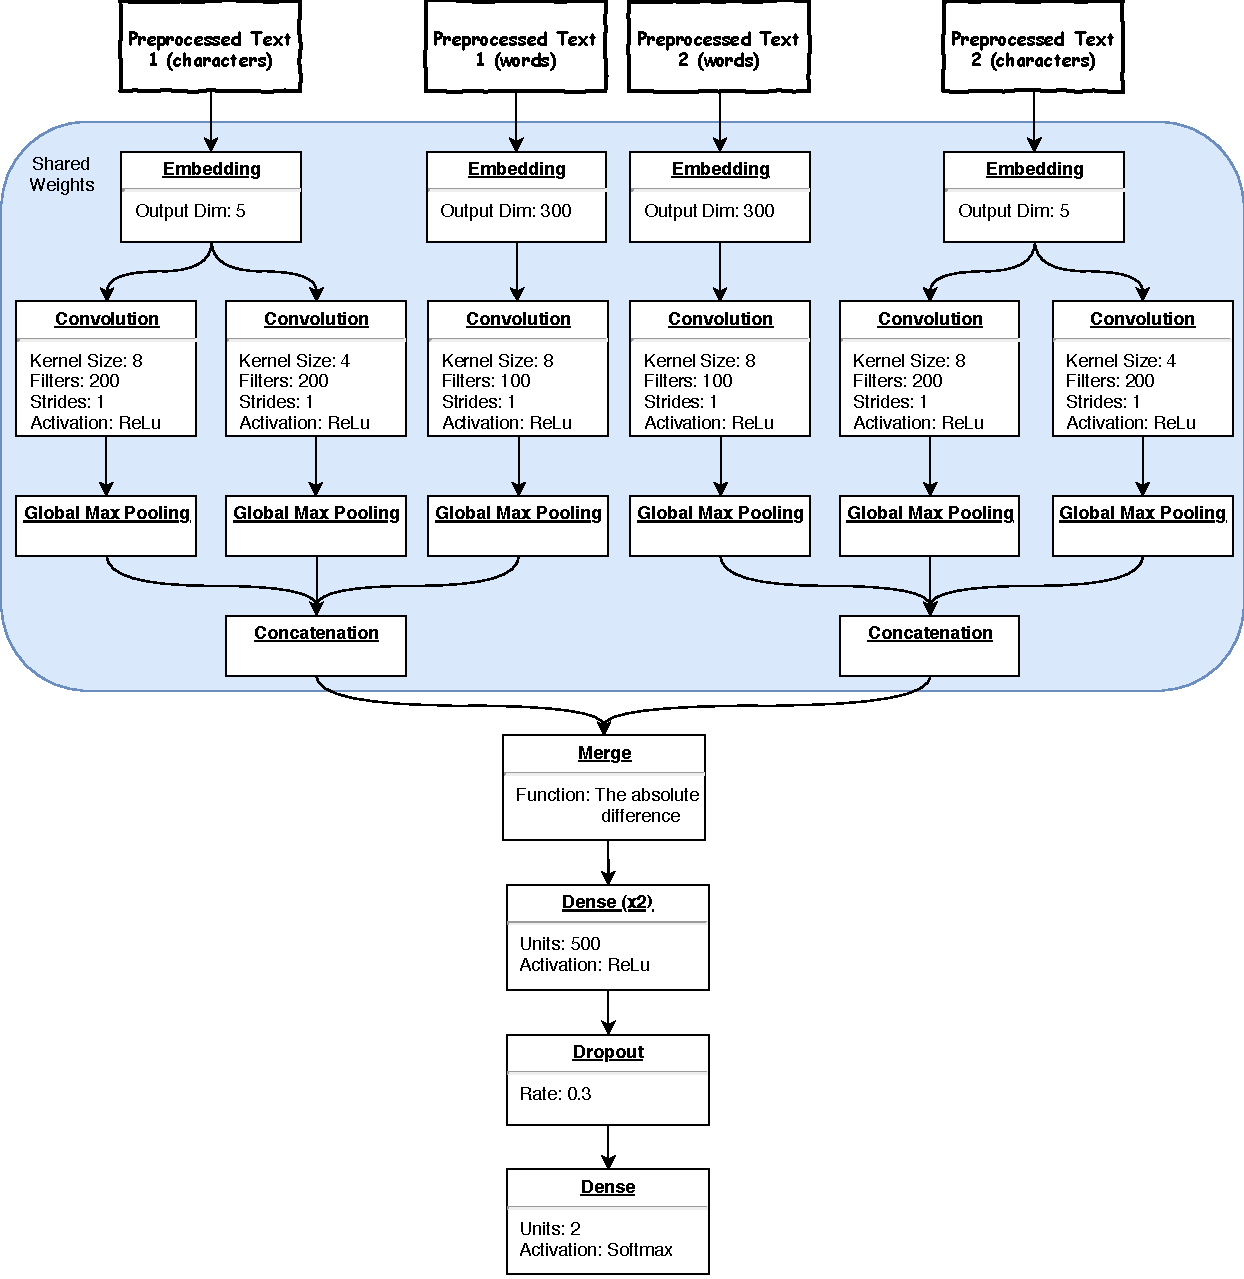
\includegraphics[width=0.7\textwidth]{../../report/pictures/experiments/conv_char_word_nn/model}
    %\end{center}
%\end{frame}

\begin{frame}[fragile]{Combining Network Output}
    \begin{itemize}
        \item We combine the output of the network using a weighted average.
        % TODO: Continue.
    \end{itemize}
\end{frame}

\begin{frame}[fragile]{Results}
    % TODO
\end{frame}

\begin{frame}[fragile]{Teacher Feedback}
    \begin{center}
        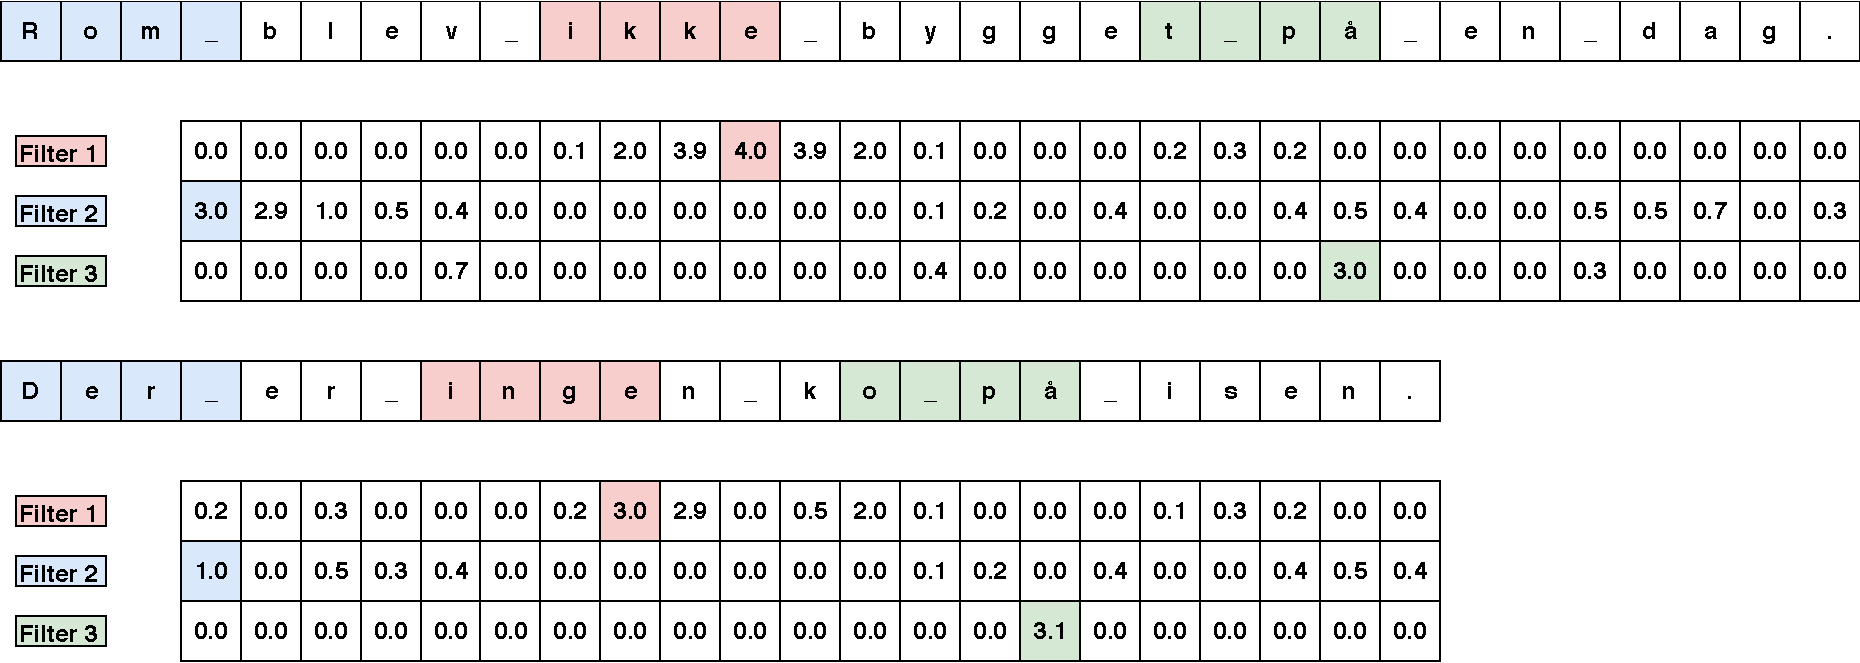
\includegraphics[width=\textwidth]{../../report/pictures/discussion/teacher_feedback_example}
    \end{center}
\end{frame}

\begin{frame}[fragile]{Teacher Feedback}
    \begin{center}
        \scriptsize
        \begin{tabular}{lll|lll}
            \textbf{Max 1}    & \textbf{Max 2}    & \textbf{Max 3}       &
            \textbf{Text 1}   & \textbf{Text 2}   & \textbf{Difference}  \\
            \hline
            \verb[nemlig 1[   & \verb[nemlig 1[   & \verb[nemlig –[      &
            \verb'pere.\n\nH' & \verb'nemlig b'   & |3.06 - 4.70| = 1.64 \\

            \verb[, F.eks.[   & \verb[, F.eks.[   & \verb[, F.eks.[      &
            \verb'. F.eks.'   & \verb'del. Und'   & |4.73 - 3.18| = 1.55 \\

            \verb[ke …''. [   & \verb[a...''\n\n[ & \verb[n''. '' [      &
            \verb'v. Men d'   & \verb'n. Den v'   & |4.28 - 2.91| = 1.37 \\

            \verb[forsøger[   & \verb[forsøger[   & \verb[forsøger[      &
            \verb'for sætt'   & \verb'forsøgte'   & |3.40 - 4.77| = 1.37 \\

            \verb[, Hvorda[   & \verb[, Hvorda[   & \verb[,08 – 6,[      &
            \verb', som ti'   & \verb', Hvorda'   & |3.70 - 5.07| = 1.37 \\

            \verb[der; ’’M[   & \verb[der; ”Ha[   & \verb[der; ”Ma[      &
            \verb'dem; Nia'   & \verb'der omha'   & |4.64 - 3.28| = 1.36 \\

            \verb[. Her ef[   & \verb[. Her ef[   & \verb[' Her br[      &
            \verb'. Jeg vi'   & \verb'. Her fo'   & |2.61 - 3.92| = 1.31 \\

            \verb[r dog kr[   & \verb[r dog kr[   & \verb[r dog ’d[      &
            \verb'r og lud'   & \verb'r dog i '   & |2.83 - 4.13| = 1.30 \\

            \verb[11], da [   & \verb[:1], da [   & \verb[:1], da [      &
            \verb'ys”, der'   & \verb'for, da '   & |3.78 - 5.04| = 1.26 \\

            \verb[, så Car[   & \verb[, så Car[   & \verb[, så Car[      &
            \verb', så er '   & \verb', som En'   & |5.19 - 3.94| = 1.25 \\
            \hline
            \verb[; ’S[       & \verb[; ’S[       & \verb[; ’E[          &
            \verb'; Ni'       & \verb'r He'       & |3.12 - 1.78| = 1.34 \\

            \verb[; ”t[       & \verb[; ”t[       & \verb[; ”t[          &
            \verb'; ”H'       & \verb', ”j'       & |3.44 - 2.13| = 1.31 \\

            \verb[d.’ [       & \verb[d.’ [       & \verb[d.’ [          &
            \verb'ne-V'       & \verb'20’e'       & |1.75 - 2.77| = 1.02 \\

            \verb[1\n’’[      & \verb[1]’’[       & \verb[1]’’[          &
            \verb' l2-'       & \verb'720’'       & |1.75 - 2.71| = 0.96 \\

            \verb['Det[       & \verb['Det[       & \verb['Det[          &
            \verb'ndet'       & \verb' Det'       & |2.37 - 3.25| = 0.88 \\

            \verb[f 1"[       & \verb[f 1"[       & \verb[f 1"[          &
            \verb'f 2\n'      & \verb'v og'       & |3.05 - 2.20| = 0.85 \\

            \verb[æk''[       & \verb[’’ é[       & \verb[ud;'[          &
            \verb'lv; '       & \verb',tro'       & |2.60 - 1.77| = 0.83 \\

            \verb[\n\nx\n[    & \verb[\n\nx\n[    & \verb[\n\nx\n[       &
            \verb'\n\n\n\n'   & \verb'\n\n5\n'    & |1.81 - 2.61| = 0.80 \\
            \verb[ “… [       & \verb[ “… [       & \verb[?“! [          &
            \verb'nd” '       & \verb'r,” '       & |1.75 - 2.53| = 0.78 \\

            \verb[S\n, [      & \verb[S\n, [      & \verb[O\n, [         &
            \verb'e\n, '      & \verb'ad, '       & |2.62 - 1.92| = 0.70 \\
        \end{tabular}
    \end{center}
\end{frame}

\begin{frame}[fragile]{Conclusion}
    \begin{itemize}
        \item Did not perform as well as MaCom wanted.
        \item Best network achieved accusation error of 23.5\% while catching
            8.5\% of ghostwriters.
        \item Better results than previous work on MaCom dataset.
        \item We believe that with further work we would be able to get below
            the 10\% accusation error while catching 10-20\% of cheaters.
        \item Almost suceeded on a 50\% ghostwritten dataset with an accusation
            error of 9.9\% while catching 82.1\% of the ghostwriters.
        \item Able to give teachers feedback.
    \end{itemize}
\end{frame}

\end{document}
